\chapter{Evaluation des risques}

\section{Identification des risques}
Le premier risque rencontré   arrive dès  la première phase – celle du plan d’action WP1.2 et WP1.3 - et est celui de  la justesse de l’analyse de la situation actuelle  et de celles des besoins auxquels apporter de l’attention. Il s’agit  de la base du projet et une erreur dans cette analyse emmènerait potentiellement  le projet vers une solution inadéquate, voire insatisfaisante. Il s’agit d’un risque humain car ces erreurs trouveront leurs sources dans le manque de qualifications, de connaissances du terrain ou dans la négligence des personnes menant l’analyse. 
 
Au vu du planning, nous devons considérer aussi le risque que représente l’épidémie de grippe saisonnière (s’étalant généralement de la fin janvier jusqu’à la mi-mars) lors de la phase WP1.  Cette phase comporte beaucoup de réunions, et des  absences  imprévues pourrait engendrer du retard sur le planning. 

 

Un autre risque, du même ordre, viendra à la phase du plan marketing WP2.2  
Il s’agit à nouveau d’un risque humain car c’est celui du choix du choix de la solution par rapport aux utilisateurs cibles. Il est question d’être certain que notre projet de bornes interactives  soit bien adapté  aux personnes que l’on souhaite aider et qu’elles seront aptes et disposées à utiliser la solution proposée.  

 

Ensuite viennent les  risques de problèmes techniques lors de la phase de WP 3.2. Nous pouvons considérer : 

 \begin{itemize} 
    \item Le risque que les infrastructures soient inadaptées. Ce qui mènerait à devoir repenser une partie de la solution technique et donc à une perte de temps et  des coûts additionnels 
    
    \item Le risque de retard dans la commande des composants des bornes entrant du retard dans la suite du projet. 
    \item Le risque  que certains composants électroniques soient défectueux 

    \item Le risque que le système manque d’ergonomie ou ne soient pas assez intuitif pour le publique cible.  

    \item Le risque que les bornes se dégradent rapidement  suite  aux intempéries, à un usage non conventionnel ou à des actes de vandalisme. 

 \end{itemize}

Finalement, nous retrouvons les risques de la phase  WP 4.3, celle de la mise en place du plan de communication.  
Les utilisateurs cibles pourraient se montrer  moins  réceptifs que prévu à la campagne de communication derrière le projet –  à cause du contenu, format ou support qui serait inadapté - et donc  ils pourraient accorder un intérêt moindre au projet. 

A cela, s’ajoute des risques contextuels affectant la visibilité de la publicité autour du projet. Par exemple : Si des  affichages publicitaires avaient été placés sur le campus, avec le contexte du soudain confinement de mars, leur visibilité aurait été quasi nulle et par  extension leur intérêt aussi. 

\section{Analyse des risques}
Nous avons analysé les risques suivants selon des axes qualitatifs :  
    \begin{figure}[h]
        \centering
        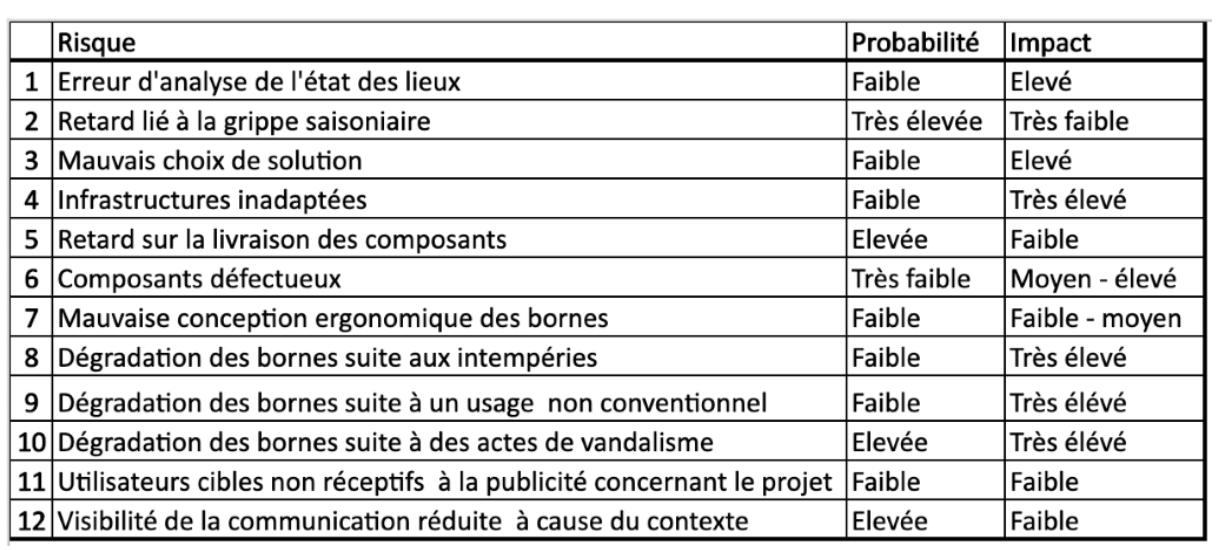
\includegraphics[width=15cm]{Pictures/analyseRisque.png}
    \end{figure}

\subsection{Matrice des risques}
    \begin{figure} [h]
        \centering
        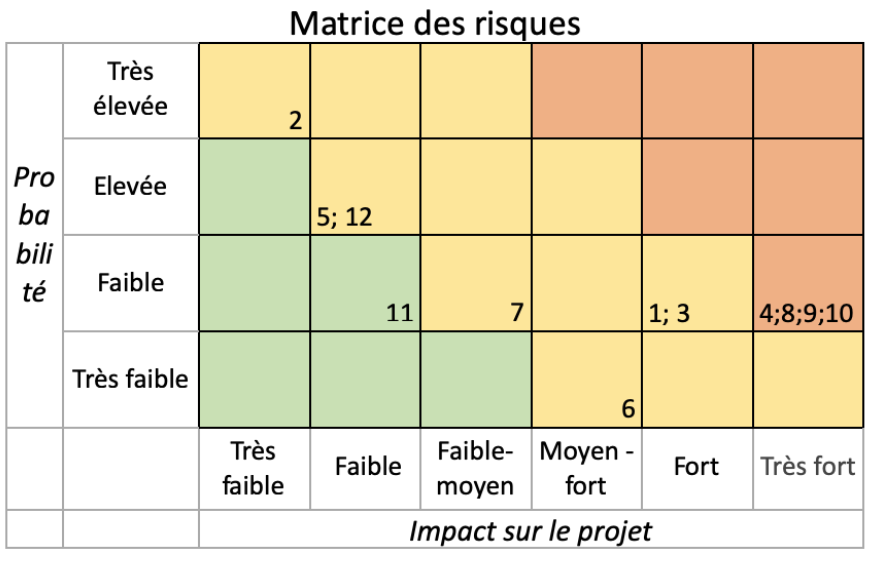
\includegraphics[width=15cm]{Pictures/matriceRisque.png}
    \end{figure}

\section{Mitigation des risques}

    \begin{figure}
        \centering
        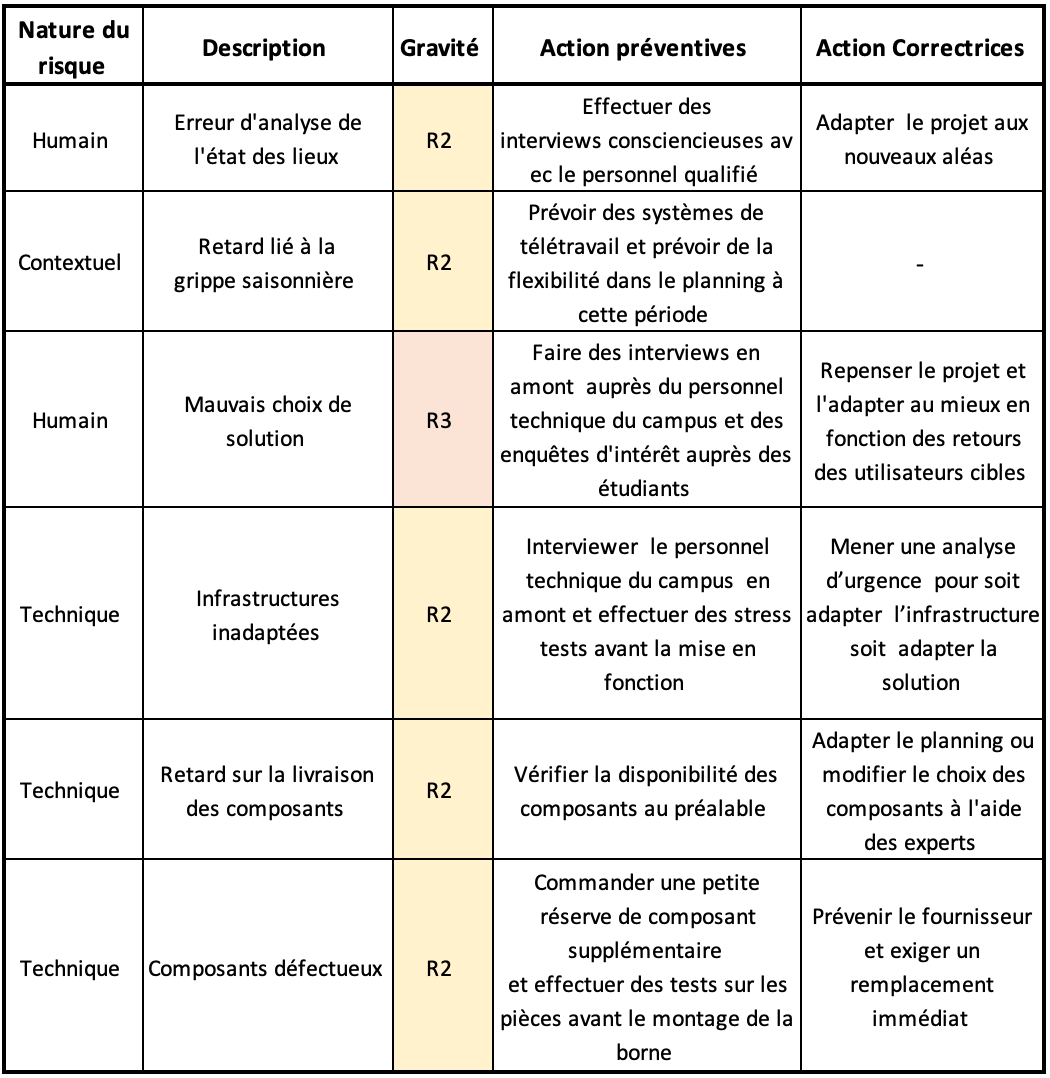
\includegraphics[width=15cm]{Pictures/mitigation1.png}
    \end{figure}

    \begin{figure}
        \centering
        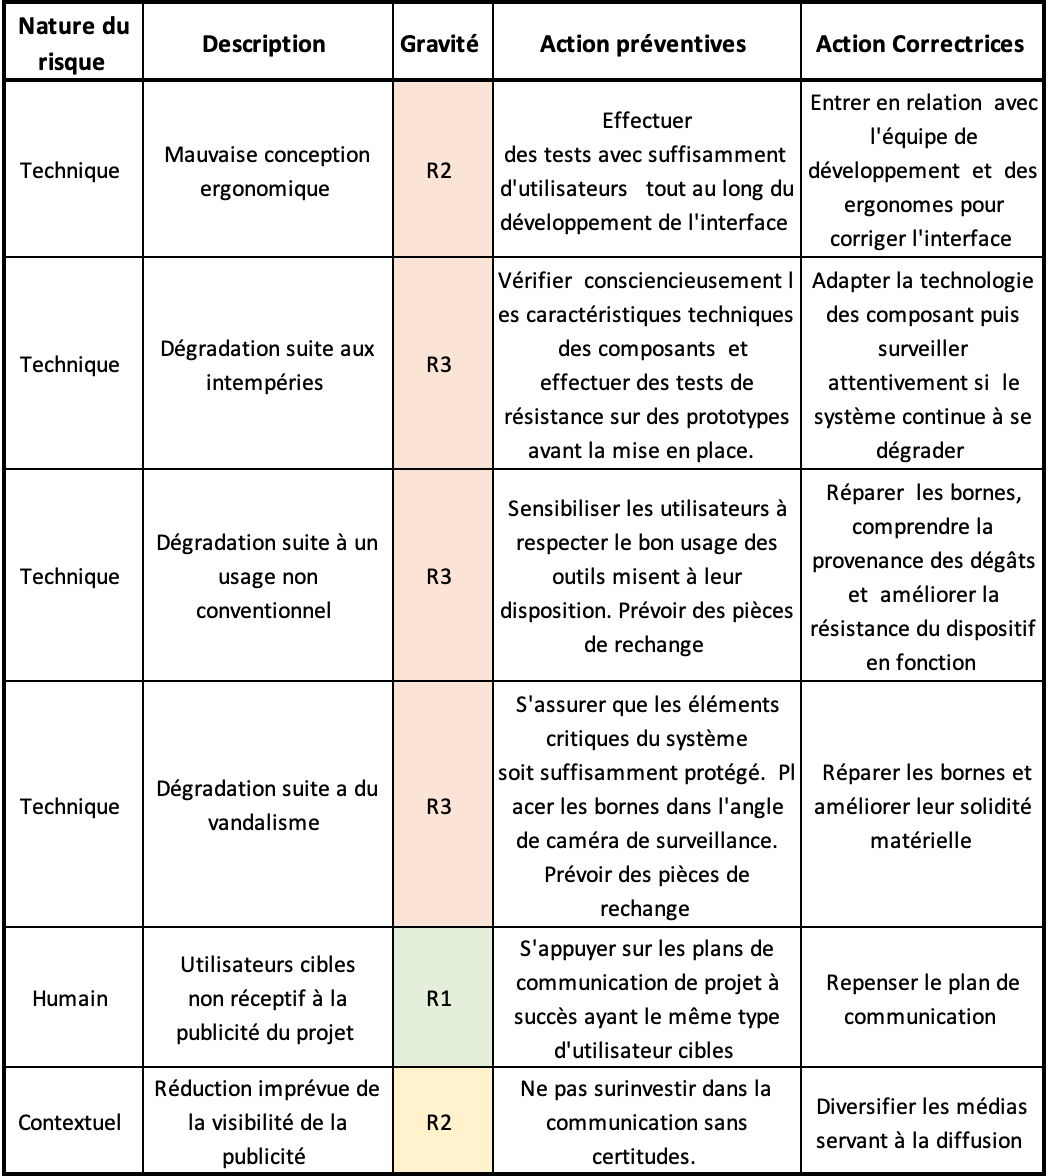
\includegraphics[width=15cm]{Pictures/mitigation2.png}
    \end{figure}
